\title{Arch Linuxのインストール}
\author{おがわ}
\begin{document}
  \begin{frame}
    \note {
      動画全体ので説明する項目概要です。\\
      1から4の項目があります。
    }
    \frametitle{Arch Linuxのインストール}
    \begin{enumerate}
      \item \alert<2>{ハードウェア、ファーム(UEFI)の仕様}
        \note [item] {
          ハードウェア、ファーム(UEFI)の仕様\\
          OSのインストーラソフト(Arch linux)は、ファーム(UEFI)の仕様に従いハードウェアを認識します。仕様を理解しておくと、動作しない場合の対策を立てやすくなります。
        }
      \item \alert<3>{OSのファイルシステム}
        \note [item] {
          OSのファイルシステム\\
          ストレージデバイス(ssd)のパーティション設定、各パーティションのファイルフォーマットの選定と設定をおこないます。
        }
      \item \alert<4>{Linuxのインストールと起動設定}
        \note [item] {
          Linuxのインストール\\
          インストーラソフトによるストレージデバイスへのLinuxカーネルと必要なソフトウェアのインストールを行います。インストールの後に起動設定を行います。
        }
      \item \alert<5>{ネットワークの接続設定}
        \note [item] {
          ネットワークの接続設定\\
          ネットワーク接続設定のためのソフトウェアの選定、インストールを行います。インストールの後にネットワークの設定を行います。
        }
    \end{enumerate} 
  \end{frame}
  \begin{frame}
    \frametitle{ハードウェア構成}
    \note{
      インストール対象のハードウェアは次のとおりです。
      裏面の蓋をあけて中身を確認していきます。
    }
    \newcommand{\selectspec}{\usebeamercolor[fg]{alerted text}}
    \begin{center}
      \begin{tabular}{l|l}
        \hline
        \temporal<2>{CPU}{\selectspec{CPU}}{CPU}%
          & \temporal<2>{AMD Ryzen7 8845HS}
            {\selectspec{AMD Ryzen7 8845HS}}
            {AMD Ryzen7 8845HS} \\ \hline
        \temporal<3>{メモリ}{\selectspec{メモリ}}{メモリ}%
          & \temporal<3>{64 GB}
            {\selectspec{64 GB}}{64 GB} \\  \hline
        \temporal<4>{SSD}{\selectspec{SSD}}{SSD}%
          & \temporal<4>{2 TB}{\selectspec{2 TB}}{2 TB} \\ \hline
        \temporal<5>{グラフィック}{\selectspec{グラフィック}}{グラフィック}%
          & \temporal<5>{Radeon 780M}
            {\selectspec{Radeon 780M}}
            {Radeon 780M} \\ \hline
      \end{tabular}
    \end{center}
    \begin{center}
      \includegraphics<1>[height=4cm, page=1]{img/hw-img.pdf}%
      \includegraphics<2,5>[height=4cm, page=13]{img/hw-img.pdf}%
      \includegraphics<3>[height=4cm, page=15]{img/hw-img.pdf}%
      \includegraphics<4>[height=4cm, page=14]{img/hw-img.pdf}%
    \end{center}
    \note[item]{cpuはAMD Ryzen7。本体の裏面の蓋を開けた状態の画像からは確認できません。} 
    \note[item]{memoy 32GBのメモリカード2枚で64GB}
    \note[item]{ストレージはssdで、2TBを設置}
    \note[item]{グラフィックはRadeon。こちらも画像からは確認できません。}
  \end{frame}
  \begin{frame}
    \frametitle{入出力ポート} 
    \note{
      入出力ポートについては、次のものが利用できます。
    }
    \newcommand{\selectspec}{\usebeamercolor[fg]{alerted text}}
    \begin{center}
      \begin{tabular}{l|l|l}
        \hline
        \temporal<1>{USB 3.2}{\selectspec{USB 3.2}}{USB 3.2}%
          & \temporal<1>{2}{\selectspec{2}}{2}%
          & \\ \hline
        \temporal<2>{USB 2.0}{\selectspec{USB 2.0}}{USB 2.0}%
          & \temporal<2>{2}{\selectspec{2}}{2} & \\ \hline
        \temporal<3>{HDMI}{\selectspec{HDMI}}{HDMI}%
          & \temporal<3>{2}{\selectspec{2}}{2} & \\ \hline
        \temporal<4>{DP}{\selectspec{DP}}{DP}%
          & \temporal<4>{2}{\selectspec{2}}{2} & \\ \hline
        \temporal<5>{シリアルポート}
            {\selectspec{シリアルポート}}{シリアルポート}%
          & \temporal<5>{1}{\selectspec{1}}{1}%
          & \temporal<5>{RS232、RS485}
            {\selectspec{RS232、RS485}}{RS232、RS485} \\ \hline
      \end{tabular}
      \note[item] {USB3.2タイプAのポートが2つ。位置は前面}
      \note[item] {USB2.0タイプAのポートが2つ。位置は背面}
      \note[item] {HDMIポートが2つ。位置は背面}
      \note[item] {ディスプレイポート2.1が2つ。位置は背面}
      \note[item] {シリアルのポートが1つ。位置は背面。今すぐの利用は考えていません。}
    \end{center}
    \begin{center}
      \includegraphics<1>[height=4cm, page=3]{img/hw-img.pdf}%
      \includegraphics<2>[height=4cm, page=4]{img/hw-img.pdf}%
      \includegraphics<3>[height=4cm, page=5]{img/hw-img.pdf}%
      \includegraphics<4>[height=4cm, page=6]{img/hw-img.pdf}%
      \includegraphics<5>[height=4cm, page=7]{img/hw-img.pdf}%
    \end{center}
  \end{frame}
  \begin{frame}
    \frametitle{ネットワーク} 
    \note{
      ネットワーク関連は、表のようになっています。
    }
    \newcommand{\selectspec}{\usebeamercolor[fg]{alerted text}}
    \begin{center}    
      \begin{tabular}{l|l}
        \hline
        \temporal<1>{イーサネット}{\selectspec{イーサネット}}{イーサネット}%
        & \temporal<1>{2}{\selectspec{2}}{2} \\ \hline
        \temporal<2>{Wi-Fi}{\selectspec{Wi-Fi}}{Wi-Fi}%
        & \temporal<2>{1}{\selectspec{1}}{1}\\
        \hline
      \end{tabular}
      \note[item] {イーサネットポートが2つ。位置は背面}
      \note[item] {Wi-Fiが1つ。アンテナが背面に確認できます}
    \end{center}
    \begin{center}
      \includegraphics<1>[height=4cm, page=8]{img/hw-img.pdf}%
      \includegraphics<2>[height=4cm, page=9]{img/hw-img.pdf}%
    \end{center}
  \end{frame}
  \begin{frame}
    \frametitle{ファーム}
    \note{
      AMI社のファームで、UEFI仕様に従っています。
      起動ボタン押下直後にF2で設定が変更できます。
      ファームについて簡単な説明をしておきます。
      ファームとはマザーボードのチップに書き込まれたソフトウェアです。ファームは、CPUやマザーボードに接続された機器との通信を行います。ファームは、基本的な機能だけを提供しています。ファームの機能を組み合わせて利用すると複雑な処理を行うことができます。\\
      ファームがUEFI仕様に従っているおかげで、汎用的にソフトウェアを開発することができます。
      このことについて、次に説明していきます。
    }
    \begin{center}
    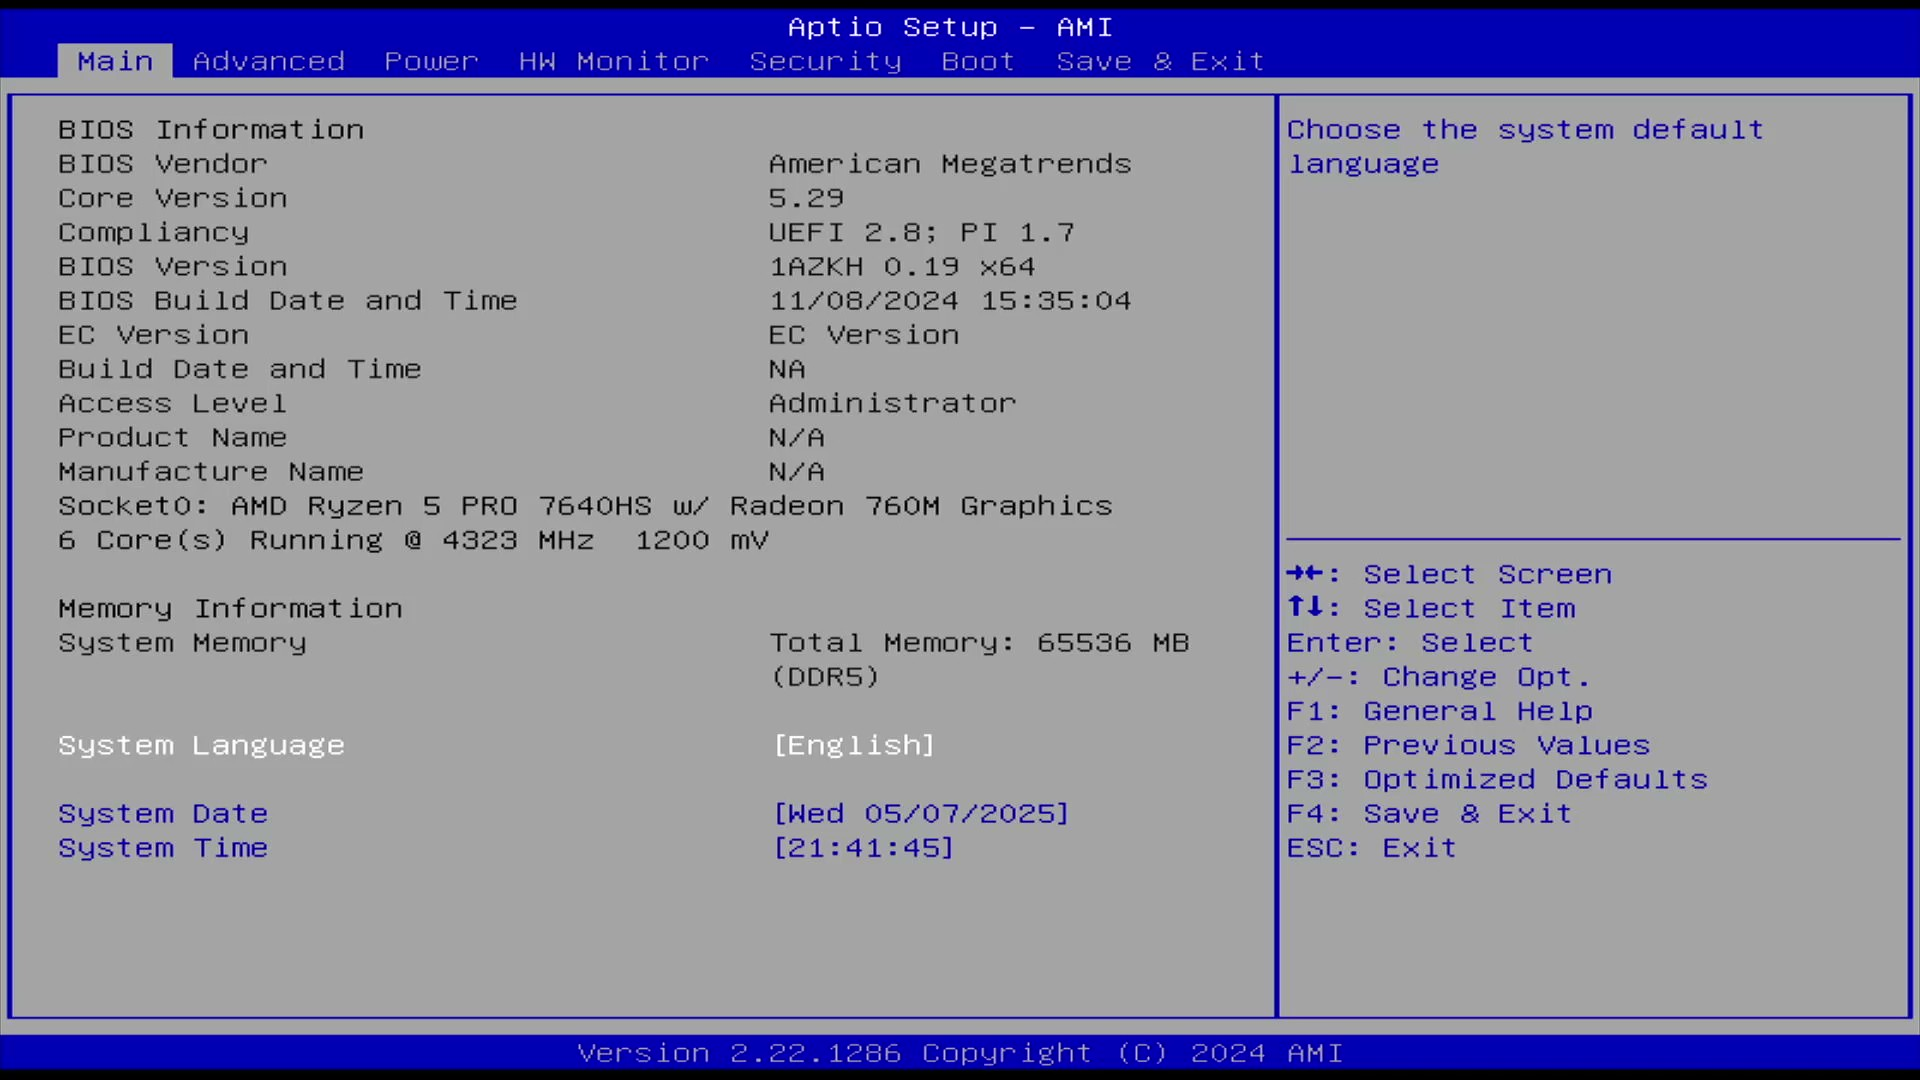
\includegraphics[height=5cm]{img/bios-display-1.jpg}
    \end{center}
  \end{frame}
  \begin{frame}
    \frametitle{要件を満たすソフトウェア}
    \note{ファームの説明のために、ユーザーの要件を満たすようなソフトウェアを開発することを考えます。}
    \only<1>{要件\\}%
    \only<2>{開発\\}%
    \only<3>{査収\\}%
    \only<4>{運用\\}%
    \only<5>{改修要件\\}%
    \only<6>{改修\\}%
    \only<7>{ソフト移行\\}%
    \begin{center}
      \includegraphics<1>[height=6cm, page=1]{img/sw-requirement.pdf}%
      \includegraphics<2>[height=6cm, page=2]{img/sw-requirement.pdf}%
      \includegraphics<3>[height=6cm, page=3]{img/sw-requirement.pdf}%
      \includegraphics<4>[height=6cm, page=4]{img/sw-requirement.pdf}%
      \includegraphics<5>[height=6cm, page=5]{img/sw-requirement.pdf}%
      \includegraphics<6>[height=6cm, page=6]{img/sw-requirement.pdf}%
      \includegraphics<7>[height=6cm, page=7]{img/sw-requirement.pdf}%
    \end{center}
    \note[item]<1>{発注者の要件を明確にします。}
    \note[item]<2>{要件を元に、ソフトウェアを開発します。
      通常は、成果物、設計、納期、テストケースなどについても、発注者と確認を取ります。ここでは割愛しています。}
    \note[item]<3>{発注者が、要件をみたしていることを確認して、受領となります。}
    \note[item]<4>{受領されたソフトウェアの運用を開始します。ここでは、発注者が運用していますが、運用は別の組織となることも多いです。}
    \note[item]<5>{実運用を始めると、当初の要件では、気付かなかった問題が生じることがあります。iPhoneアプリの応答が遅いとか\ldots  このケースでは、サーバの処理能力の向上で解決する追加要件となっています。}

    \note[item]<6>{要件を満たすサーバを選定します。}
    \note[item]<7>{現行サーバのソフトについて、新サーバでも動作させることができるのでしょうか?}  
  \end{frame}
  
  \begin{frame}
    \frametitle{ハードウェアの利用とソフトウェア}
    \note{ハードウェアを提供する組織は、独自の取り組みで、性能を向上させます。
    }
    \note[item]<1> {このため、図示のように、A社、B社、C社で異なった、ソフトウェアインターフェイスとなってしまうことも考えられます。すると、ソフトウェアの機能は同じでも、A社用、B社用、C社用のソフトウェアを用意しなければならないことになってしまいます。同じ機能のソフトのため、3種類用意するために作業するのは、時間的に効率がよいとはいえません。
    } 
    \note[item]<2>{この不都合を解決するするために、統一したソフトウェアインターフェイスとして、UEFIが提供されています。A社、B社、C社がUEFIに適合したソフトウェアインターフェースを提供することで、ハードウェアが異なっても、同一のソフトウェアで動作させることできます。}
    \alt<2>{UEFIがある}{UEFIがない}

    \includegraphics<1>[height=4cm, page=1]{img/hw-fm-sw.pdf}%
    \includegraphics<2>[height=4cm, page=2]{img/hw-fm-sw.pdf}%
    \note[item]<2>{実際には、A社、B社、C社は、統一したUEFIインターフェースを用意することになりますので、各社が負担の一部を肩代わりしているとも考えられます。}

  \end{frame}
  \begin{frame}
    \center
    作業を始めます
    \note{
      ファームまでの説明が終わりましたので、作業を開始します。
    }
  \end{frame}
  \begin{frame}
    \frametitle{iPXEのダウンロード}
    以下のURLのページからUEFI用のiPXEをダウンロード\\
    \url{https://archlinux.org/releng/netboot/}\\
    \note[item]<1>{UEFIファームが起動したあと、UEFIファームが起動する最初のソフトウェアを用意します。iPXEは、インターネットを介してインストーラソフトをダウンロードし、そのダウンロードソフトを実行するソフトウェアになります。iPXE本体をインターネットからダウンロードします。}
    \note[item]<2>{今回は、Arch Linuxをインストーラをインストールしたいので、Arch LinuxのiPXEをダウンロードします。}
    \note[item]<3>{ページの下の方に、UEFIタイトルが確認できます。}
    \note[item]<4>{リンクをクリックしてダウンロードします。}
    \begin{center}
      \includegraphics<1>[bb=0 2cm 6cm 8.61cm,clip=true, height=4cm, page=1]
        {img/ipxe-http-page.pdf}%
      \includegraphics<2>[bb=0 2cm 6cm 8.61cm,clip=true, height=4cm, page=2]
        {img/ipxe-http-page.pdf}%
      \includegraphics<3>[bb=0 2cm 4cm 5cm,clip=true, height=4cm, page=1]
        {img/ipxe-http-page.pdf}%
      \includegraphics<4>[bb=0 2cm 4cm 5cm,clip=true, height=4cm, page=3]
        {img/ipxe-http-page.pdf}%
    \end{center}
    \uncover<4->{\url{https://archlinux.org/static/netboot/ipxe-arch.efi}}
  \end{frame}
  \begin{frame}
    \frametitle{Netboot用USB作成}
    \note{
      この説明の後、実際にUSB作成の操作を、動画で実演します。環境はWindows11になっています。実演のあらましを説明します。
    }
    \begin{enumerate}
      \item<1-> USBのドライブにEFI{\textbackslash}BOOTディレクトリを作成する
      \note[item]<1>{USBのドライブにEFI{\textbackslash}BOOTディレクトリを作成します。}
      \item<2-> ipxe-arch.efiをBOOTx64.efiに変名する
      \note[item]<2>{ipxe-arch.efiをBOOTx64.efiに変名します。}
      \item<3-> BOOTx64.efiをEFI{\textbackslash}BOOTに保存する
      \note[item]<3>{BOOTx64.efiをEFI{\textbackslash}BOOTに保存します。}
    \end{enumerate} 
    \note[item]<3>{
      UEFIの仕様ではUSBフラッシュがFAT8、FAT16、FAT32のファイルシステムで、EFI{\textbackslash}BOOT.EFIがUEFIアプリケーション(BOOT loader)として認識されます。
      動画では、ipxe-arch.efiはipxe-archの後ろに16進数が続いていますが、最近のarch用のipxeのダウンロードでは、16進数がつかないようです。
    }
  \end{frame}
  \begin{frame}
    ファイルシステムの要件とlvmの説明  
  \end{frame}
  \begin{frame}
    \frametitle{ファイルシステム}
    \note {
      Arch Linuxのインストールの前にssdのファイルシステムを決定します。作成したファイルシステムに、Arch Linuxのソフトウェアをインストールします。ファイルシステムはLinuxがファイル操作をするためのものでもあるので、Linuxが認識できるファイルシステムを選定することになります。
    } 
    要件\\ 
    \begin{enumerate}
      \item<2->{lvmを使用する。}
      \item<3->{ext4ファイルシステムを使用する。}
      \item<4->{スワップパーティションは作成せず、スワップファイルを作成する。}
    \end{enumerate}
    \note[item]<2>{lvmは、後ほど説明します。}
    \note[item]<3>{ファイルシステムについて、ext4で問題を感じたことがないので、ext4を使用します。}
    \note[item]<4>{スワップサイズを事前決定することは、難しいので、パーティションを作成せずにスワップファイルで、必要に応じて変更する運用とします。}
  \end{frame}
  \begin{frame}
    \frametitle{lvmとは}
    \note{
      Logical Volume Manager通称lvmとは、複数のストレージ、パーティションをまとめて、一つの論理的な領域として、使用できるようなソフトウェアです。
    }
    複数のストレージを一つの領域にすることができる   
    \begin{center}
      \includegraphics<1>[height=4cm, page=1]
        {img/lvm.pdf}%
      \includegraphics<2>[height=4cm, page=2]
        {img/lvm.pdf}%
    \end{center}
    \note[item]<1>{lvmを使用しない場合は、パーティション毎に容量が分割されます。}
    \note[item]<2>{lvmを使用すると、分割された容量を大きな容量にをまとまった容量として使用することができます。}
  \end{frame} 
  \begin{frame}
    \frametitle{lvmの利点}
    \note{
      lvmの利点について、理解するため、ファイルシステムへのデータ保存について考えます。
    }
    \alt<1-8>{lvmなし}{lvmあり}
    \begin{center}
      \includegraphics<1>[height=5cm, page=1]
        {img/lvm-usecase.pdf}%
      \includegraphics<2>[height=5cm, page=2]
        {img/lvm-usecase.pdf}%
      \includegraphics<3>[height=5cm, page=3]
        {img/lvm-usecase.pdf}%
      \includegraphics<4>[height=5cm, page=4]
        {img/lvm-usecase.pdf}%
      \includegraphics<5>[height=5cm, page=5]
        {img/lvm-usecase.pdf}%
      \includegraphics<6>[height=5cm, page=6]
        {img/lvm-usecase.pdf}%
      \includegraphics<7>[height=5cm, page=7]
        {img/lvm-usecase.pdf}%
      \includegraphics<8>[height=5cm, page=8]
        {img/lvm-usecase.pdf}%
      \includegraphics<9>[height=5cm, page=9]
        {img/lvm-usecase.pdf}%
      \includegraphics<10>[height=5cm, page=10]
        {img/lvm-usecase.pdf}%
      \includegraphics<11>[height=5cm, page=11]
        {img/lvm-usecase.pdf}%
      \includegraphics<12>[height=5cm, page=12]
        {img/lvm-usecase.pdf}%
      \includegraphics<13>[height=5cm, page=13]
        {img/lvm-usecase.pdf}%
      \includegraphics<14>[height=5cm, page=14]
        {img/lvm-usecase.pdf}%
      \includegraphics<15>[height=5cm, page=15]
        {img/lvm-usecase.pdf}%
      \includegraphics<16>[height=5cm, page=16]
        {img/lvm-usecase.pdf}%
      \includegraphics<17>[height=5cm, page=17]
        {img/lvm-usecase.pdf}%
      \includegraphics<18>[height=5cm, page=18]
        {img/lvm-usecase.pdf}%
    \end{center}
    \note[item]<1>{ssdにデータが保存されている状態を想定します。ファイルシステムはext4としています。}
  
    \note[item]<2>{データを追加する必要が出てきました。}
    \note[item]<3-4>{空き容量よりも、追加のデータの方が大きい見込みです。}
    \note[item]<5>{ssdを増設します。}
    \note[item]<6-7>{増設したsdd側にファイルシステムを設定し、追加データを保存します。}   
    \note[item]<8>{継続して、システムを使用しているとデータを追加する必要がでてきました。増設前、増設後のssdのいずれにも空き容量があります。どちらに保存して運用するのがよいか、迷う場面も多いです。将来どの程度データが増えるかとか見通しをたてる必要があったりする場合もありますが、見通しを立てにくい場合もあると思います。} 

    \note[item]<9>{lvmを導入した場合について、同様にデータ保存されている状態を想定します。}
    \note[item]<10>{データを追加する必要が出てきました。}
    \note[item]<11-12>{空き容量よりも、追加のデータの方が大きい見込みです。}
    \note[item]<13>{ssdを追加します。}
    \note[item]<14>{physical volume(物理ボリューム)をssdに作成します。}
    \note[item]<15>{physical volumeを使用中のlogical volumeに追加します。}
    \note[item]<16>{ファイルシステム(ext4)の使用可能領域をlogical volumeに合わせて拡大します。}
    \note[item]<17-18>{データを追加します。lvmがある場合は、ボリュームが分割されていないので、保存先について迷う必要がなくなります。}
  \end{frame}
  \begin{frame}
    \frametitle{ssdのパーティションとファイルシステム構成}
    \begin{center}
      \includegraphics<1>[width=11cm, page=1]
        {img/linux-fs.pdf}%
      \includegraphics<2>[width=11cm, page=3]
        {img/linux-fs.pdf}%
      \includegraphics<3>[width=11cm, page=2]
        {img/linux-fs.pdf}%
      \includegraphics<4>[width=11cm, page=4]
        {img/linux-fs.pdf}%
    \end{center}  
    \note[item]<1>{ssdのファイルシステムを図示のようにします。}
    \note[item]<2>{LinuxのApiを利用するソフトウェア側からは、ext4がファイルシステムになります。}
    \note[item]<3>{ext4はlvmの仮想ボリューム上に作成されます。}
    \note[item]<4>{FAT32は、UEFIファームがLinuxカーネルをロードするソフトウェアを格納します。OSをロードするソフトウェアはBootLoaderと呼ばれたりします。}
  \end{frame}
  \newpage
  \begin{frame}
    \frametitle{fdiskによるssdのパーティション}
    
    \begin{center}
      \includegraphics<1>[width=11cm, page=1]
        {img/storage-part.pdf}%
      \includegraphics<2>[width=11cm, page=2]
        {img/storage-part.pdf}%
      \includegraphics<3>[width=11cm, page=3]
        {img/storage-part.pdf}%
      \includegraphics<4>[width=11cm, page=4]
        {img/storage-part.pdf}%
      \includegraphics<5>[width=11cm, page=5]
        {img/storage-part.pdf}%
      \only<6>{
        \scriptsize
        \begin{tabular}{|p{2.4cm}|r|r|p{4cm}|}
          \hline
          名前 & 位置 & 長さ & 説明 \\
          \hline
          boot Code & 0 & 440
            & UEFIでは使用しません。後方互換 \\
          \hline
          Unique MBR Disk Signature & 440 & 4
            & UEFIでは使用しません。後方互換\\
          \hline
          Unknown & 444 & 2
            & UEFIでは使用しません。後方互換 \\
          \hline
          Partition Record & 446 & 16 * 4
            & MBR形式のパーティションレコード。 \\
          \hline
          Signature & 510 & 2 & 0xAA55が記録されます。\\
          \hline
          Reserved & 512 & 可変長
            & パーティションの残りの領域で、予約領域。0で埋められます。\\
          \hline
        \end{tabular}
      }% 
    \end{center} 
    \note[item]<1>{Arch Linuxのインストールガイドでは、UEFI systemパーティションに1GiBを割りあてることを推奨しています。
推奨に従い、UEFI systemパーティションは1GiBとします。

    }
    \note[item]<2>{
      残りは全て、lvmパーティションとしファイルシステムをext4にします。
    }
    \note[item]<3>{
      図示では、先頭、わずかに隙間があります。
    }
    \note[item]<4>{
      ここは、Protective MBRになっています。
      Protective MBRから始まる、パーティション情報を格納する領域を確保するため、 最初のGTPパーティションが2048 セクター(2048 x 512 byte)の位置から始まることになります。ここは、UEFIが登場する前の起動シーケンスで利用されたデータ形式が残っていると考えてよいと思います。
    }
    \note[item]<5>{データ開始位置0で始まる部分なので、どうなっているか気になりましたので、調べてみました。実運用では、重要な部分はないと思います。
    }
    \note[item]<6>{表のなかでは、Partition Recordが活用されているデータとなっています。4つのパーティションレコードが格納できますが、最初の1つのみが使用されます。
最初の1つが、Protective MBRに後続するGPT Headerを指しています。
GPT Headerに続き、GTP Pertition Entry Arrayが続きます。GTP Pertition Entry Arrayの各エントリーが、各パーティションの開始位置と、終了位置を記録しています。
    }
  \end{frame}
\end{document}
% vi: se ts=2 sw=2 et:
